\chapter{Metodologia e Desenvolvimento do Sistema}

\section{Arquitetura Geral do Sistema}

O simulador desenvolvido neste trabalho foi implementado como uma aplicação \textit{web} executada integralmente no navegador do usuário, permitindo sua utilização sem a necessidade de instalação de softwares adicionais.


\subsection{Tecnologias Utilizadas}

A aplicação foi desenvolvida utilizando as seguintes tecnologias:

\begin{itemize}
    \item \textbf{HTML}: responsável pela estruturação dos elementos da interface;
    \item \textbf{CSS}: utilizado para organização visual e disposição dos componentes na página;
    \item \textbf{JavaScript}: empregado na implementação da lógica do sistema;
    \item \textbf{Babylon.js}: biblioteca gráfica baseada em WebGL utilizada para renderização tridimensional e manipulação da cena;
    \item \textbf{Chart.js}: biblioteca utilizada para geração dos gráficos de posição, velocidade e aceleração das juntas.
\end{itemize}

Toda a execução ocorre no lado do cliente (\textit{client-side}), sendo o navegador responsável tanto pelo processamento matemático quanto pela renderização gráfica em tempo real.

\subsection{Estrutura do Sistema}

O código foi organizado de forma modular, separando responsabilidades específicas em diferentes arquivos:

\begin{itemize}
    \item \texttt{index.html}: define a estrutura da interface e os elementos visuais;
    \item \texttt{scene.js}: implementa a criação da cena 3D, modelagem do manipulador e controle das juntas;
    \item \texttt{aux\_func.js}: contém as funções matemáticas auxiliares, incluindo rotinas relacionadas à cinemática inversa;
    \item \texttt{grafico.js}: responsável pela configuração e atualização dos gráficos.
\end{itemize}

Essa divisão favorece a organização do código, facilita a manutenção e permite maior clareza na separação entre interface gráfica, modelagem matemática e visualização.

\subsection{Fluxo de Funcionamento}

O funcionamento do sistema segue o seguinte fluxo geral:

\begin{enumerate}
    \item O usuário interage com a interface por meio de controles deslizantes ou comandos de execução de trajetória;
    \item As variáveis articulares são atualizadas conforme a entrada fornecida;
    \item A nova configuração do manipulador é aplicada à estrutura hierárquica da cena 3D;
    \item A pose do efetuador final é recalculada e, quando aplicável, utilizada na atualização dos gráficos;
    \item O motor gráfico renderiza a cena atualizada em tempo real.
\end{enumerate}

Esse processo ocorre dentro do laço de renderização do motor gráfico, garantindo atualização contínua da cena e dos elementos gráficos.

\subsection{Sistema de Coordenadas e Estrutura Hierárquica}

A cena tridimensional foi configurada utilizando um sistema de coordenadas de mão direita, com o eixo $z$ orientado verticalmente, em concordância com a modelagem cinemática adotada.

A estrutura do manipulador foi implementada por meio de uma hierarquia de nós (\textit{TransformNodes}), em que cada junta é modelada como um elemento pai do elo subsequente. Dessa forma, as transformações aplicadas a uma junta propagam-se automaticamente para os elos descendentes, reproduzindo computacionalmente a cadeia cinemática aberta descrita na fundamentação teórica.

Essa abordagem permite que o comportamento geométrico do manipulador seja obtido por meio do encadeamento das transformações locais, equivalente ao produto sucessivo das matrizes homogêneas apresentado no Capítulo 2.

\section{Modelagem do Manipulador}

A modelagem do manipulador foi conduzida com o objetivo de garantir coerência entre a estrutura geométrica adotada, a formulação cinemática apresentada no Capítulo 2 e a implementação computacional desenvolvida no simulador. A escolha da configuração geométrica precedeu a modelagem tridimensional, de modo que o modelo CAD refletisse fielmente as características cinemáticas desejadas.

\subsection{Definição da Geometria}

O manipulador desenvolvido é do tipo serial com seis graus de liberdade, composto exclusivamente por juntas revolutas (configuração 6R). A escolha de seis graus de liberdade deve-se ao fato de que a pose completa de um corpo rígido no espaço tridimensional é definida por seis parâmetros independentes: três associados à posição e três à orientação. Dessa forma, um manipulador 6R permite o posicionamento e orientação arbitrários do efetuador final dentro de seu espaço de trabalho.

Além disso, foi adotada a configuração com punho esférico, na qual os três últimos eixos de rotação intersectam-se em um único ponto. Essa característica geométrica é fundamental para a solução analítica da cinemática inversa, pois permite o desacoplamento entre o problema de posicionamento e o problema de orientação, conforme discutido na Seção 2.5.

Nessa abordagem, as três primeiras variáveis articulares determinam a posição do centro do punho, enquanto as três últimas variáveis são responsáveis exclusivamente pela orientação do efetuador final. Essa propriedade reduz a complexidade matemática do problema inverso e viabiliza a obtenção de soluções fechadas, tornando o sistema mais eficiente para execução em tempo real.

% =====================================================
% FIGURA DO ESQUEMA CINEMÁTICO (AINDA A SER INSERIDA)
% =====================================================
%
% AQUI SERÁ INSERIDA UMA FIGURA DO ESQUEMA CINEMÁTICO
% DO MANIPULADOR, COM IDENTIFICAÇÃO DAS JUNTAS (J1–J6)
% E DOS EIXOS DE ROTAÇÃO.
%
% Sugestão:
% \begin{figure}[H]
%     \centering
%     \includegraphics[width=0.8\textwidth]{Imagens/Esquema_Cinematico_6R.png}
%     \caption{Esquema cinemático do manipulador 6R com identificação das juntas e eixos de rotação.}
%     \label{fig:esquema_cinematico}
% \end{figure}
%
% =====================================================

\subsection{Parâmetros Cinemáticos do Manipulador}

Com base na geometria definida, foram estabelecidos os parâmetros de Denavit--Hartenberg correspondentes a cada elo, conforme apresentado no Capítulo 2. A atribuição dos sistemas de coordenadas foi realizada de modo consistente com a configuração 6R e com a interseção dos eixos no punho esférico.

A definição adequada desses parâmetros garante que a modelagem matemática represente corretamente a estrutura física do manipulador, permitindo que o produto sucessivo das transformações homogêneas reproduza o comportamento geométrico observado na representação tridimensional.

\begin{table}[H]
\centering
\caption{Parâmetros de Denavit--Hartenberg do manipulador 6R}
\label{tab:DH_parametros}
\begin{tabular}{c c c c c}
\hline
\textbf{i} & $\boldsymbol{\alpha_i}$ (°) & $\boldsymbol{a_i}$ (mm) & $\boldsymbol{d_i}$ (mm) & $\boldsymbol{\theta_i}$ \\ 
\hline
1 & 90  & 100 & 330 & $\theta_1$ \\
2 & 0   & 400 & 0   & $\theta_2$ \\
3 & -90 & 0   & 0   & $\theta_3$ \\
4 & 90  & 0   & 375 & $\theta_4$ \\
5 & -90 & 0   & 0   & $\theta_5$ \\
6 & 0   & 0   & 200 & $\theta_6$ \\
\hline
\end{tabular}
\end{table}

\subsection{Modelagem CAD e Exportação}

O modelo mecânico do manipulador foi desenvolvido na plataforma Onshape, ferramenta de modelagem CAD baseada em nuvem. Cada elo foi modelado individualmente, respeitando as dimensões adotadas na definição dos parâmetros cinemáticos e priorizando a clareza estrutural do conjunto.

Foram modelados os principais elementos estruturais do manipulador, incluindo base, elos intermediários e efetuador final. Elementos secundários, como parafusos ou componentes internos não relevantes para a análise cinemática, não foram incluídos, a fim de manter o modelo computacionalmente leve e adequado para execução em ambiente \textit{web}.

\begin{figure}[H]
    \centering
    
\includegraphics[width=0.85\textwidth]{Imagens/OnShape_Assembly.png}
    \caption{Modelo CAD do manipulador serial 6R desenvolvido no Onshape.}
    \label{fig:OnShape_Assembly}
\end{figure}

Após a modelagem, os componentes foram exportados no formato STL. Esses arquivos foram importados para o ambiente tridimensional da aplicação \textit{web}, onde foram realizados ajustes de orientação inicial e posicionamento relativo, garantindo alinhamento com a estrutura cinemática implementada.

\subsection{Correspondência entre Modelo Geométrico e Modelo Cinemático}

Após a importação dos arquivos STL, foi estabelecida a correspondência entre cada componente geométrico e sua respectiva junta na estrutura hierárquica do sistema. Para cada elo foi definido um nó de transformação associado ao eixo de rotação correspondente, garantindo que as rotações aplicadas no ambiente computacional reproduzissem fielmente a modelagem baseada nos parâmetros DH.

Essa integração entre o modelo geométrico e o modelo matemático assegura consistência entre a representação visual do manipulador e o comportamento cinemático descrito teoricamente, permitindo que o simulador mantenha coerência entre análise matemática e visualização tridimensional.

\begin{figure}[H]
    \centering
    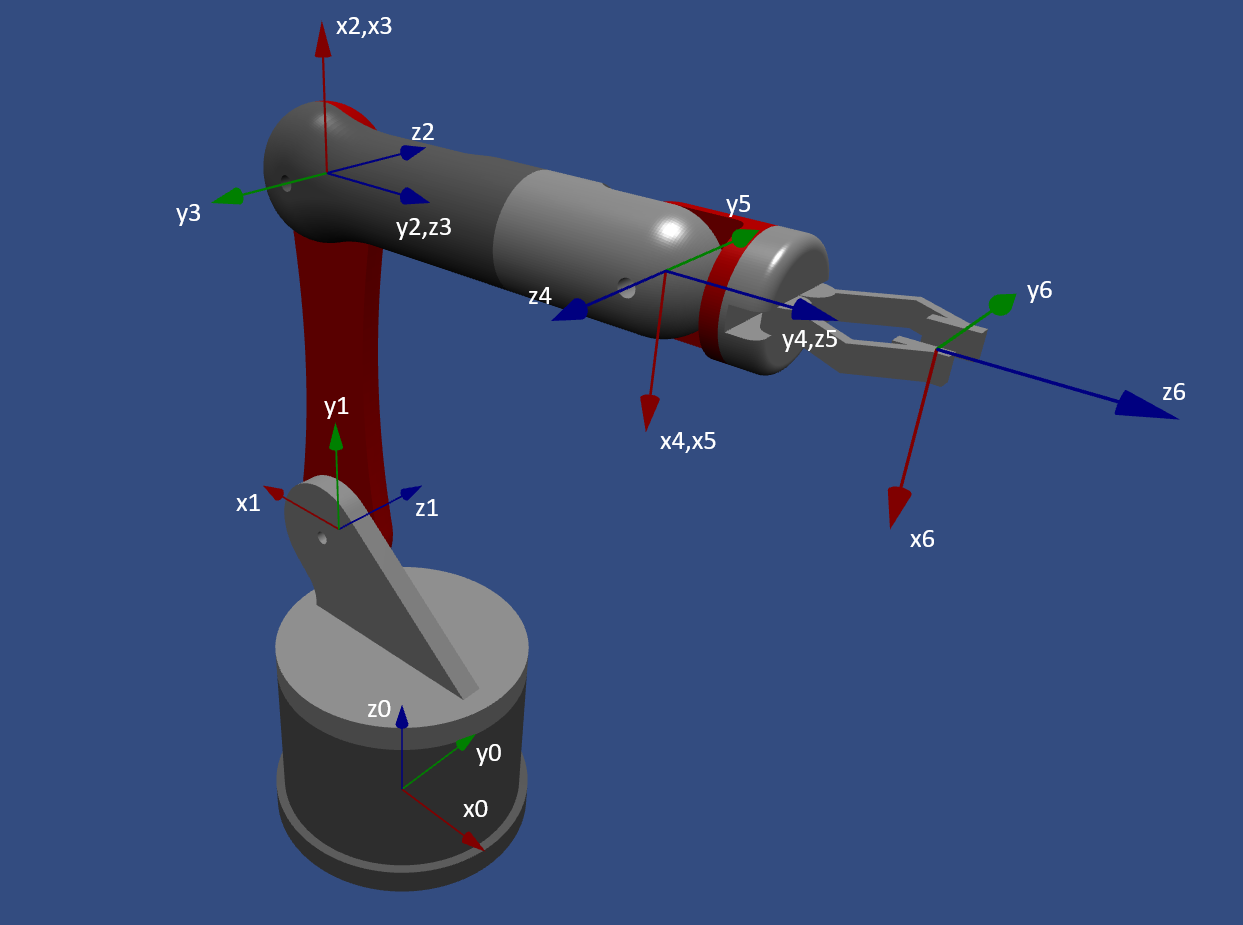
\includegraphics[width=0.85\textwidth]{Imagens/render_eixos.png}
    \caption{Renderização do manipulador no ambiente de simulação, com visualização dos eixos locais associados às juntas.}
    \label{fig:render_eixos}
\end{figure}

\section{Implementação da Cinemática Direta}

A implementação da cinemática direta no simulador segue a formulação apresentada no Capítulo 2, na qual a pose do efetuador final é obtida pelo produto sucessivo das matrizes de transformação homogênea associadas a cada elo do manipulador.

No ambiente computacional, essa operação não é implementada explicitamente por meio da multiplicação das matrizes DH. Em vez disso, ela é realizada implicitamente pelo motor gráfico Babylon.js por meio da estrutura hierárquica de transformações da cena tridimensional. Nessa estrutura, cada junta do manipulador é representada por um nó de transformação, de modo que as rotações aplicadas às juntas propagam-se automaticamente ao longo da cadeia cinemática, produzindo o mesmo efeito geométrico descrito pelo modelo matemático.

\subsection{Estratégia de Implementação}

Cada junta do manipulador foi associada a um nó de transformação (\textit{TransformNode}), responsável por aplicar a rotação correspondente à variável articular. Os elos geométricos importados em formato STL foram vinculados a esses nós, de modo que as transformações aplicadas a uma junta afetassem automaticamente todos os elos subsequentes.

Essa estrutura pai–filho reproduz computacionalmente a cadeia cinemática aberta descrita teoricamente. Assim, a rotação aplicada à junta $i$ é acumulada com as transformações das juntas anteriores, produzindo o mesmo efeito geométrico que o produto sucessivo das matrizes homogêneas:

\begin{equation}
^0\mathbf{T}_n = \prod_{i=1}^{n} \, ^{i-1}\mathbf{T}_i
\end{equation}

Dessa forma, a hierarquia da cena tridimensional atua como uma implementação direta do modelo matemático.

\subsection{Atualização das Variáveis Articulares}

O controle das variáveis articulares no simulador é realizado por meio de elementos de interface do tipo \textit{slider}, associados individualmente a cada uma das seis juntas do manipulador. Cada controle deslizante permite a definição direta do valor angular correspondente à variável $\theta_i$, dentro de limites previamente estabelecidos para cada junta.

\begin{figure}[H]
    \centering
    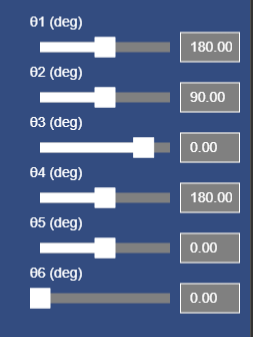
\includegraphics[width=0.3\textwidth]{Imagens/slider.png}
    \caption{\textit{Sliders} para controle do manipulador no espaco de juntas}
    \label{fig:slider}
\end{figure}

Os valores fornecidos pelos \textit{sliders} são definidos em graus para facilitar a interação do usuário. Internamente, esses valores são convertidos para radianos antes de serem aplicados às rotações locais dos respectivos nós de transformação, garantindo compatibilidade com as funções trigonométricas utilizadas pelo motor gráfico.

Sempre que ocorre uma alteração no valor de um \textit{slider}, o sistema atualiza imediatamente a rotação associada à junta correspondente. Como os elos estão organizados em uma estrutura hierárquica, a modificação de uma junta é automaticamente propagada aos elos subsequentes, refletindo instantaneamente na postura global do manipulador.

Essa atualização ocorre dentro do laço de renderização da aplicação, permitindo resposta visual em tempo real. Dessa forma, o usuário pode observar imediatamente o efeito de cada variação angular, o que reforça o caráter didático do simulador e evidencia a relação direta entre as variáveis articulares e a configuração espacial do manipulador.

\subsection{Obtenção da Matriz do Efetuador}

Embora a multiplicação explícita das matrizes homogêneas não seja realizada manualmente no código, a matriz de transformação global do efetuador final é obtida diretamente a partir da estrutura hierárquica da cena tridimensional.

Para isso, utiliza-se a função \texttt{getWorldMatrix()} do motor gráfico Babylon.js, aplicada ao nó correspondente ao efetuador final. Essa função retorna a matriz de transformação acumulada do objeto em relação ao sistema de referência global da cena, incorporando todas as rotações e translações herdadas da cadeia de nós pais.

Após sua obtenção, a matriz é organizada no formato $4 \times 4$ e exibida na interface do simulador, na região inferior da tela. Essa atualização ocorre em tempo real, acompanhando continuamente as variações impostas às juntas, seja por meio dos \textit{sliders} ou durante a execução de trajetórias programadas.

Dessa forma, o usuário pode observar simultaneamente a movimentação tridimensional do manipulador e a correspondente matriz de transformação homogênea, reforçando a relação entre a modelagem matemática apresentada no Capítulo 2 e o comportamento geométrico do sistema implementado.

\section{Implementação da Cinemática Inversa}

A implementação da cinemática inversa no simulador foi realizada por meio de uma solução analítica baseada no desacoplamento entre posição e orientação, viabilizada pela configuração de punho esférico adotada na geometria do manipulador.

\subsection{Estratégia de Desacoplamento}

Conforme discutido na Seção 2.5, a interseção dos três últimos eixos de rotação permite separar o problema da cinemática inversa em duas etapas independentes:

\begin{enumerate}
    \item Determinação das três primeiras variáveis articulares a partir da posição do centro do punho;
    \item Determinação das três últimas variáveis a partir da orientação desejada do efetuador final.
\end{enumerate}

Essa abordagem reduz significativamente a complexidade do problema, evitando a necessidade de métodos numéricos iterativos.

\subsection{Cálculo do Centro do Punho}

Seja $^0\mathbf{T}_6$ a transformação homogênea desejada do efetuador final. A posição do centro do punho pode ser obtida subtraindo-se o deslocamento do último elo ao longo do eixo $z_6$:

\begin{equation}
\mathbf{p}_w = \mathbf{p} - d_6 \mathbf{R} \hat{z}
\end{equation}

onde $\mathbf{p}$ representa a posição do efetuador, $\mathbf{R}$ sua orientação e $d_6$ o deslocamento associado ao último elo.

A partir da posição $\mathbf{p}_w = (x_w, y_w, z_w)$, determina-se inicialmente a variável $\theta_1$ por meio da projeção no plano $xy$:

\begin{equation}
\theta_1 = \arctan2(y_w, x_w)
\end{equation}

As variáveis $\theta_2$ e $\theta_3$ são obtidas por meio da resolução do triângulo formado pelos elos 2 e 3, utilizando a Lei dos Cossenos. Seja:

\begin{equation}
r = \sqrt{x_w^2 + y_w^2}
\end{equation}

\begin{equation}
s = z_w - d_1
\end{equation}

Define-se então:

\begin{equation}
D = \frac{r^2 + s^2 - a_2^2 - a_3^2}{2 a_2 a_3}
\end{equation}

de onde:

\begin{equation}
\theta_3 = \arctan2(\pm\sqrt{1-D^2}, D)
\end{equation}

e

\begin{equation}
\theta_2 = \arctan2(s, r) - \arctan2(a_3 \sin\theta_3, a_2 + a_3 \cos\theta_3)
\end{equation}

O sinal associado à raiz quadrada determina diferentes configurações geométricas possíveis, como as posições de ``cotovelo para cima'' ou ``cotovelo para baixo''.

\subsection{Determinação das Variáveis do Punho}

Uma vez determinadas as três primeiras variáveis articulares, calcula-se a matriz de rotação associada aos três primeiros elos:

\begin{equation}
^0\mathbf{R}_3
\end{equation}

A matriz de rotação do punho é então obtida por:

\begin{equation}
^3\mathbf{R}_6 = (^0\mathbf{R}_3)^T \, ^0\mathbf{R}_6
\end{equation}

A partir dessa matriz, as variáveis $\theta_4$, $\theta_5$ e $\theta_6$ são extraídas utilizando as relações trigonométricas correspondentes aos elementos de $^3\mathbf{R}_6$.

O código completo referente à implementação dessas etapas encontra-se no Anexo A.

\subsection{Interface de Controle Cartesiano}

Além do controle direto das variáveis articulares, o simulador disponibiliza um modo alternativo de operação baseado em coordenadas cartesianas.

Nesse modo, o usuário define diretamente:

\begin{itemize}
    \item Posição: $x$, $y$, $z$;
    \item Orientação: \textit{yaw}, \textit{pitch} e \textit{roll}.
\end{itemize}

\begin{figure}[H]
    \centering
    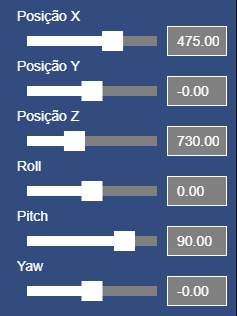
\includegraphics[width=0.3\textwidth]{Imagens/slider_ci.png}
    \caption{\textit{Sliders} para controle do manipulador no espaço cartesiano}
    \label{fig:slider_ci}
\end{figure}

Os valores de orientação são convertidos em uma matriz de rotação $^0\mathbf{R}_6$ por meio da composição das rotações elementares associadas aos ângulos de Euler adotados.

A partir da transformação homogênea desejada, o algoritmo de cinemática inversa é executado, retornando o vetor de variáveis articulares correspondente. Esses valores são então automaticamente aplicados aos \textit{sliders} articulares, atualizando instantaneamente a postura do manipulador.

Essa integração permite alternar entre controle no espaço das juntas e controle no espaço cartesiano, reforçando o caráter didático da ferramenta e evidenciando a relação entre as duas representações.

\section{Tratamento de Singularidades}

Durante a resolução da cinemática inversa, determinadas configurações geométricas do manipulador podem levar a situações conhecidas como singularidades. Nessas configurações, ocorre perda de mobilidade em determinadas direções do espaço operacional, tornando o cálculo das variáveis articulares indeterminado ou numericamente instável.

Em termos gerais, singularidades estão associadas à perda de posto da matriz Jacobiana do manipulador. Nessas situações, pequenas variações na pose desejada do efetuador podem resultar em variações muito grandes nas variáveis articulares, ou mesmo tornar impossível a obtenção de uma solução única.

No manipulador adotado neste trabalho, a singularidade mais relevante ocorre no punho esférico, quando os eixos das juntas 4 e 6 tornam-se colineares. Essa condição ocorre quando:

\begin{equation}
\sin(\theta_5) = 0
\end{equation}

ou, equivalentemente,

\begin{equation}
\theta_5 = 0 \quad \text{ou} \quad \theta_5 = \pi
\end{equation}

Nessa configuração, o sistema perde um grau de liberdade de orientação, pois rotações em torno das juntas 4 e 6 passam a produzir o mesmo efeito no efetuador final. Consequentemente, a determinação individual dos ângulos $\theta_4$ e $\theta_6$ torna-se indeterminada.

Para evitar instabilidades numéricas durante a execução do algoritmo de cinemática inversa, foi implementado um tratamento específico para situações em que o valor de $\sin(\theta_5)$ se aproxima de zero. Nesses casos, o algoritmo identifica a proximidade da singularidade e adota uma estratégia de regularização, mantendo uma solução consistente para as variáveis articulares e evitando variações abruptas na configuração do manipulador.

Esse tratamento garante continuidade no movimento do manipulador durante a execução das trajetórias e contribui para a estabilidade da simulação em tempo real.
\section{Implementação do Planejamento de Trajetória}

O simulador desenvolvido permite a programação de trajetórias para o manipulador, possibilitando a execução automática de movimentos entre diferentes configurações articulares. Conforme discutido na Seção 2.6, o planejamento de trajetória foi implementado por meio de interpolação polinomial cúbica no espaço das juntas.

Nesse modo de operação, o usuário pode registrar uma sequência de configurações articulares intermediárias que devem ser atingidas ao longo do movimento. Para cada etapa da trajetória, é definido também o intervalo de tempo necessário para a transição entre duas configurações consecutivas.

\subsection{Definição dos Pontos da Trajetória}

Os pontos da trajetória são definidos diretamente a partir da configuração atual do manipulador. Ao registrar um novo ponto, o sistema armazena os valores das variáveis articulares correspondentes, bem como o tempo de execução associado ao deslocamento até o próximo ponto.

Dessa forma, cada segmento da trajetória é definido por um par de configurações articulares consecutivas e pelo intervalo de tempo necessário para a transição entre elas.

\subsection{Cálculo dos Coeficientes do Polinômio}

Para cada junta do manipulador, os coeficientes do polinômio cúbico são calculados a partir das posições inicial e final do movimento e do tempo total definido para o segmento da trajetória. Conforme apresentado na Seção 2.6, são consideradas velocidades nulas nos instantes inicial e final do movimento, garantindo suavidade na transição entre os pontos programados.

Os coeficientes calculados são então utilizados para determinar a evolução temporal das variáveis articulares durante a execução do movimento.

\subsection{Execução Temporal do Movimento}

Durante a execução da trajetória, o sistema calcula continuamente os valores das variáveis articulares em função do tempo decorrido desde o início do segmento em execução. Esses valores são aplicados diretamente às juntas do manipulador, atualizando sua configuração no ambiente tridimensional.

A atualização ocorre dentro do laço de renderização da aplicação, permitindo que o movimento seja exibido de forma contínua e suave na visualização gráfica.

\subsection{Geração dos Gráficos de Movimento}

A partir do polinômio cúbico utilizado para descrever a posição articular ao longo do tempo, também são obtidas as expressões de velocidade e aceleração por meio de derivação temporal.

Considerando a trajetória articular definida por:

\begin{equation}
q(t) = a_0 + a_1 t + a_2 t^2 + a_3 t^3
\end{equation}

a velocidade angular é obtida pela primeira derivada temporal:

\begin{equation}
\dot{q}(t) = a_1 + 2a_2 t + 3a_3 t^2
\end{equation}

e a aceleração angular pela segunda derivada:

\begin{equation}
\ddot{q}(t) = 2a_2 + 6a_3 t
\end{equation}

Durante a execução da trajetória, essas grandezas são calculadas continuamente para cada junta e utilizadas para alimentar os gráficos exibidos na interface do simulador. Dessa forma, o usuário pode visualizar simultaneamente os perfis temporais de posição, velocidade e aceleração das variáveis articulares ao longo do movimento programado.

\subsection{Visualização da Trajetória Espacial}

Durante a execução do movimento programado, o simulador registra sucessivamente as posições do efetuador final no espaço tridimensional. Esses pontos são utilizados para construir uma linha que representa o caminho percorrido pelo efetuador ao longo da trajetória.

Essa visualização permite observar de forma intuitiva o deslocamento espacial do manipulador durante a execução do movimento, complementando as informações fornecidas pelos gráficos das variáveis articulares.

\section{Interface Gráfica e Visualização}

A interface gráfica do simulador foi desenvolvida com o objetivo de permitir a interação direta do usuário com o manipulador, conciliando controle operacional, visualização tridimensional e acompanhamento em tempo real das grandezas cinemáticas. A disposição dos elementos na tela foi organizada de modo a facilitar tanto o uso da ferramenta em contexto didático quanto a observação simultânea do comportamento geométrico e matemático do sistema.

\subsection{Organização da Tela}

A interface principal do simulador é dividida em duas regiões principais. A região superior é destinada à visualização tridimensional do manipulador, enquanto a região inferior concentra os elementos auxiliares de interação e análise, como gráficos, dados e instruções de uso.

Essa organização permite que o usuário acompanhe continuamente a movimentação do manipulador no ambiente 3D ao mesmo tempo em que observa informações numéricas e gráficas associadas ao movimento executado.

Para permitir maior foco na visualização do movimento, a região inferior da interface pode ser minimizada pelo usuário. Dessa forma, a área dedicada à renderização tridimensional é ampliada, facilitando a observação detalhada do comportamento geométrico do manipulador durante a execução de trajetórias ou durante a manipulação direta das juntas.

\subsection{Modos de Controle}

O simulador disponibiliza dois modos principais de controle do manipulador: controle no espaço das juntas e controle no espaço cartesiano.

No modo de controle por juntas, a interface apresenta um conjunto de \textit{sliders}, cada um associado a uma variável articular do manipulador. Por meio desses controles, o usuário pode alterar diretamente os valores angulares das seis juntas, observando instantaneamente o efeito dessas variações sobre a postura do manipulador no ambiente tridimensional.

No modo de controle cartesiano, o usuário pode definir diretamente a pose desejada do efetuador final. Nesse caso, a interface disponibiliza controles deslizantes para as coordenadas espaciais $x$, $y$ e $z$, bem como para os ângulos de orientação \textit{yaw}, \textit{pitch} e \textit{roll}. 

Sempre que um desses parâmetros é alterado, o algoritmo de cinemática inversa é executado automaticamente, calculando o conjunto de variáveis articulares correspondente à pose especificada. Os valores resultantes são então aplicados ao manipulador, atualizando imediatamente sua configuração.

A possibilidade de alternância entre os dois modos de operação permite ao usuário explorar tanto o comportamento individual das juntas quanto a relação entre o espaço articular e o espaço cartesiano, contribuindo para o caráter didático da ferramenta.
\subsection{Programação de Trajetórias}

A interface também permite a definição de trajetórias por meio do registro sequencial de pontos. O usuário pode posicionar o manipulador em uma configuração desejada e armazená-la como parte de uma rotina de movimento. Para cada ponto registrado, é possível definir o tempo de transição até o próximo ponto da sequência.

Uma vez definida a rotina, o simulador executa automaticamente o movimento interpolado entre os pontos armazenados, segundo a metodologia descrita na Seção 3.6. A interface disponibiliza ainda comandos para iniciar, interromper e limpar a trajetória programada.

\subsection{Gráficos de Movimento}

Na região inferior da interface, o simulador apresenta três gráficos principais, correspondentes às variáveis de posição, velocidade e aceleração das seis juntas do manipulador. Esses gráficos são atualizados em tempo real durante a execução de uma trajetória programada.

A visualização simultânea dessas grandezas permite acompanhar não apenas a evolução angular das juntas, mas também a suavidade do movimento gerado, contribuindo para a compreensão do comportamento cinemático do sistema.

\subsection{Exibição da Matriz de Transformação}

A interface disponibiliza ainda uma área específica para exibição da matriz de transformação homogênea global do efetuador final. Essa matriz é atualizada continuamente conforme o manipulador se movimenta, permitindo que o usuário associe diretamente a postura observada na cena tridimensional à sua representação matemática.

Esse recurso amplia o caráter pedagógico do simulador ao aproximar a formulação teórica da observação prática do movimento.

\subsection{Visualização Tridimensional}

A região principal da tela é dedicada à visualização tridimensional do manipulador, implementada com recursos de câmera orbital, iluminação e renderização em tempo real. O usuário pode alterar o enquadramento da cena, aproximar ou afastar a câmera e observar o manipulador sob diferentes perspectivas.

Adicionalmente, a interface permite a exibição dos eixos locais associados às juntas, facilitando a compreensão da estrutura cinemática e da orientação de cada grau de liberdade. Durante a execução de trajetórias, também é possível observar a linha correspondente ao caminho percorrido pelo efetuador final no espaço.
